%\documentclass[10pt]{article}
%%\usepackage[utf8]{inputenc}
%%\usepackage[T1]{fontenc}
%\usepackage{amsmath}
%\usepackage{amsfonts}
%\usepackage{amssymb}
%%\usepackage[version=4]{mhchem}
%%\usepackage{stmaryrd}
%\usepackage{graphicx}
%%\usepackage[export]{adjustbox}
%%\graphicspath{ {./images/} }
%
%%\usepackage{polyglossia}
%\usepackage{latexsym}
%%\usepackage[cp1251]{inputenc}
%\usepackage[T2A,T1]{fontenc}
%%\setmainlanguage{russian}
%%\setotherlanguages{russian}
%\usepackage[russian,english]{babel}


\documentclass[12pt,a4paper]{article}
\usepackage{latexsym}
%\usepackage[cp1251]{inputenc}
%\usepackage[T2A,T1]{fontenc}
\usepackage[utf8]{inputenc}
\usepackage[russian,english]{babel}
\usepackage{amsmath,amsthm,amsfonts}
\usepackage[normalem]{ulem}
\usepackage{graphicx}

\begin{document}

\selectlanguage{english}
\noindent\textbf{Card T46}
\medskip  
\selectlanguage{russian}

\textbf{Задача: }Точки \( A_1, B_1, C_1 \) на сторонах остроугольного треугольника \( ABC \) выбраны так, что отрезки \( AA_1, BB_1, CC_1 \) пересеклись в точке \( O \), а углы \( AA_1C, BB_1A, CC_1B \) оказываютсяались равными. Докажите, что эти отрезки являются высотами треугольника \( \triangle ABC \).

\medskip
%\selectlanguage{russian}
\noindent \underline{Подсказка:}
%\selectlanguage{english}

\textbf{Доказательство:} 
Нетрудно доказать, что около четырехугольников \( AC_1OB_1 \) и \( CA_1OB_1 \) можно описать окружности. По теореме о секущей и касательной имеем равенство:
$BB_1 \cdot BO=BC \cdot BA_1 = BA \cdot BC_1$ или
$BC : BA = BC_1 : BA_1$.

Из последнего равенства следует, что \( \triangle BCC_1 \sim \triangle BAA_1 \), т.е., \( \angle BA_1A = \angle BC_1C = \angle AA_1C = 90^\circ \), т.к. углы \( BA_1A\) и \( \angle AA_1C \) являются смежными.

\bigskip
\selectlanguage{english}
\noindent\textbf{Card T47}
\medskip  
\selectlanguage{russian}

\begin{enumerate}
	\item \(\tg{\alpha} = -\frac{5}{12}\) \quad Найти \(\sin{\alpha}\) и \(\cos{\alpha}\).
	
	\medskip
	%\selectlanguage{russian}
	\noindent \underline{Подсказка:}
	%\selectlanguage{english}
$	\sin{\alpha} = \pm \frac{5}{13}, \quad \cos{\alpha} = \pm \frac{12}{13}$.

	\item \(\tg{\alpha} = -\frac{1}{2}\) \quad Найти \(\sin{\alpha}\) и \(\cos{\alpha}\).
	
	\medskip
	%\selectlanguage{russian}
	\noindent \underline{Подсказка:}
	%\selectlanguage{english}
$	\sin{\alpha} = \pm \frac{1}{\sqrt{5}}, \quad \cos{\alpha} = \pm \frac{2}{\sqrt{5}}$.

	\item \(\tg{\alpha} = -\frac{7}{4}\) \quad Найти \(\sin{\alpha}\) и \(\cos{\alpha}\).
	
	\medskip
	%\selectlanguage{russian}
	\noindent \underline{Подсказка:}
	%\selectlanguage{english}
$	\sin{\alpha} = \pm \frac{7}{5}, \quad \cos{\alpha} = \pm \frac{4}{5}$.

	\item \(\tg{\alpha} = -\frac{2}{3}\) \quad Найти \(\sin{\alpha}\) и \(\cos{\alpha}\).
	
	\medskip
	%\selectlanguage{russian}
	\noindent \underline{Подсказка:}
	%\selectlanguage{english}
$	\sin{\alpha} = \pm \frac{2}{\sqrt{13}}, \quad \cos{\alpha} = \pm \frac{3}{\sqrt{13}}$.
\end{enumerate}

\bigskip
\selectlanguage{english}
\noindent\textbf{Card T48}
\medskip  
\selectlanguage{russian}

\textbf{Задача:} Найти \(\cos(\vec{a} \cdot \vec{b})\), если \(\vec{a}\) и \(\vec{b}\) заданы векторами:
\begin{enumerate}
	\item \(\vec{a} = (1, 2)\), \(\vec{b} = (-2, 1)\)
		
	\medskip
	%\selectlanguage{russian}
	\noindent \underline{Подсказка:}
	%\selectlanguage{english}
$	\cos(\vec{a} \cdot \vec{b}) = 0$.

	\item \(\vec{a} = (-3, 2)\), \(\vec{b} = (2, 3)\)
		
	\medskip
	%\selectlanguage{russian}
	\noindent \underline{Подсказка:}
	%\selectlanguage{english}
$	\cos(\vec{a} \cdot \vec{b}) = 0$.

	\item \(\vec{a} = (4, 4)\), \(\vec{b} = (-4, -4)\)
		
	\medskip
	%\selectlanguage{russian}
	\noindent \underline{Подсказка:}
	%\selectlanguage{english}
$	\cos(\vec{a} \cdot \vec{b}) = -1$.

	\item \(\vec{a} = (-5, -5)\), \(\vec{b} = (5, 5)\)
		
	\medskip
	%\selectlanguage{russian}
	\noindent \underline{Подсказка:}
	%\selectlanguage{english}
$	\cos(\vec{a} \cdot \vec{b}) = -1$.
\end{enumerate}

\bigskip
\selectlanguage{english}
\noindent\textbf{Card T53}
\medskip  
\selectlanguage{russian} 
\begin{enumerate}
	\item \( |x + 2| = 2(3 - x); \)
	\item \( |3x - 2| + x = 10; \)
	\item \( |5x - 4| = 4 - 5x; \)
	\item \( |2x - 3| = 3 - 2x; \)
\end{enumerate}

\medskip
%\selectlanguage{russian}
\noindent \underline{Подсказка:}
%\selectlanguage{english}

\[
\begin{array}{ll}
	8, & \frac{4}{3}; \\
	-4, & 3; \\
	\frac{4}{5}, & 0.8; \\
	\frac{3}{2}, & 1.5
\end{array}
\]

\bigskip
\selectlanguage{english}
\noindent\textbf{Card T55}
\medskip  
\selectlanguage{russian} 

Найдите все натуральные числа в десятичной записи, которые уменьшаются до 1996 при вычитании из них этого числа без последней цифры.

\medskip
%\selectlanguage{russian}
\noindent \underline{Подсказка:}
%\selectlanguage{english}

Пусть число имеет вид \( \overline{abc\ldots mn} \), тогда:
\[
\overline{abc\ldots mn} - \overline{abc\ldots m} = 1996 \implies 10x + n - x = 1996 \implies 9x + n = 1996\implies
\]
\[\implies x = \frac{1996 - n}{9}, \textrm{ \ где \ }  n \in \{0, 1, \ldots, 9\}\implies
\begin{array}{l}
\left\{\begin{array}{l}
n=7\\
x=221		
\end{array}\right.
\end{array} 
\]
Ответ: \( \overline{abc\ldots mn} = 2217 \).

\bigskip
\selectlanguage{english}
\noindent\textbf{Card T59}
\medskip  
\selectlanguage{russian}

Докажите неравенство:
\[
(1 + a + a^2 + a^3)^2 \leq 4(1 + a^2 + a^4 + a^6)
\]

\medskip
%\selectlanguage{russian}
\noindent \underline{Подсказка:}
%\selectlanguage{english}		
\[
\begin{array}{l}
	\implies 3a^6 - 2a^5 + a^4 - 4a^3 + a^2 - 2a + 3 \geq 0	\implies\\
	\implies a^4(a^2 - 2a + 1) + (a^2 - 2a + 1) + 2(a^6 - 2a^3 + 1) =\\	
	=	(a^4 + 1)(a-1)^2 + 2 (a^3-1)^2 \geq 0	.
\end{array}
\]	

\bigskip
\selectlanguage{english}
\noindent\textbf{Card TD 04 (Demidova)}
\medskip
\selectlanguage{russian}

	Ученики Петя, Коля, Вася, Иван, Миша по очереди выполнили по одному примеру из таблицы умножения. При этом, у каждого последующего получился результат в полтора раза больший, чем у предыдущего. Какие числа перемножил Иван?

\underline{Подсказка:}

$$x,  \frac{3x}{2},  \frac{9x}{4}, \frac{27x}{8}, \frac{81x}{16}  \implies  x=16$$
$$16, 24, 36, 54, 81$$

\bigskip
\selectlanguage{english}
\noindent\textbf{Card TD 20 (Demidova)}
\medskip
\selectlanguage{russian}

Два брата продали $n$ цыплят по  $n$ лей. Деньги делили так. 10 лей взял старший брат, 10 лей младший, опять 10 лей старший и т.д. В конце меньшему брату не хватило денег до 10 лей. Он взял остаток и ножик старшего брата, после чего они согласились, что деление было правильным. Сколько стоит ножик?

\underline{Подсказка:}

Ясно, что выручка была $n^2$, причем, $n^2>30$. Пусть $n=10a+b$. Тогда $n^2=100a^2+20ab+b^2=20a(5a+b)+b^2$. Но число десяток в $n^2$ должно быть нечетным. Это возможно тогда и только тогда, когда $b^2=16$ или $36$. Значит, остаток равен 6. Значит, ножик стоит 2 лея. (???4 - ред.)


\bigskip
\noindent\textbf{Card T Fig 01}
\medskip
\selectlanguage{russian}

Окружность, описанная около треугольника $ABC$, пересекает продолжение медианы $BM$ в точке $D$. Докажите, что $AB\cdot AD=CB\cdot CD$.

\underline{Подсказка:}
\begin{center}
	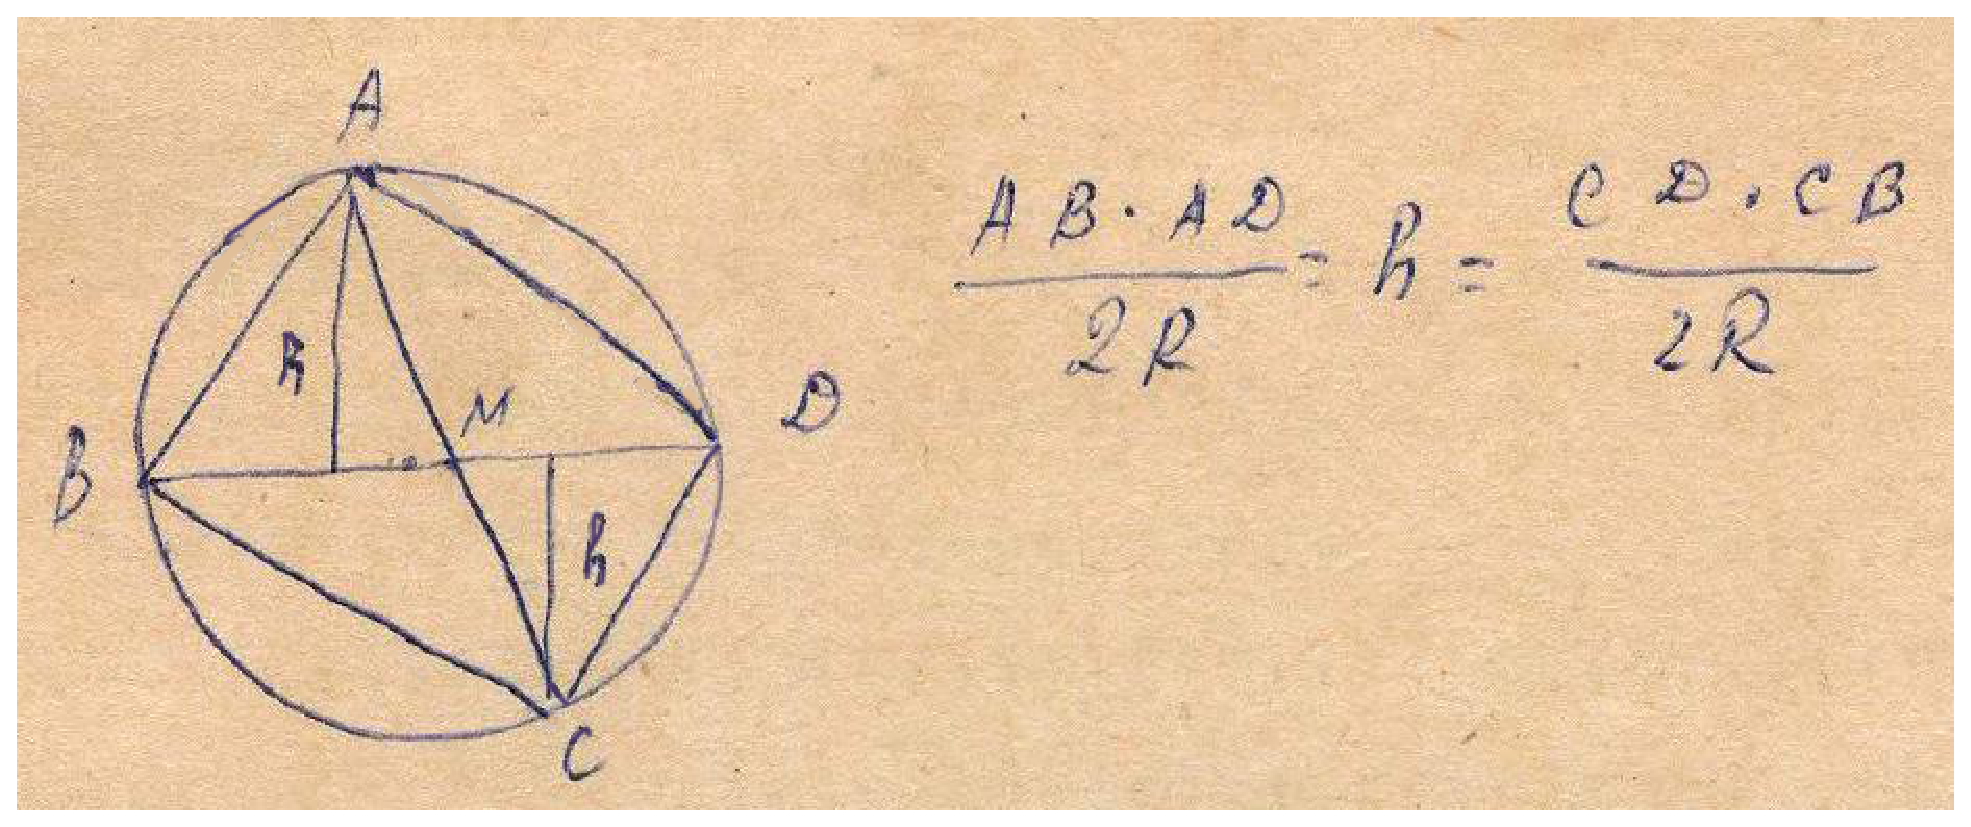
\includegraphics[width=\textwidth]{Card_T_Fig1_1.eps}
\end{center}

\bigskip
\selectlanguage{english}
\noindent\textbf{Card T Fig 06}
\medskip
\selectlanguage{russian}

\noindent \begin{minipage}{6cm}
	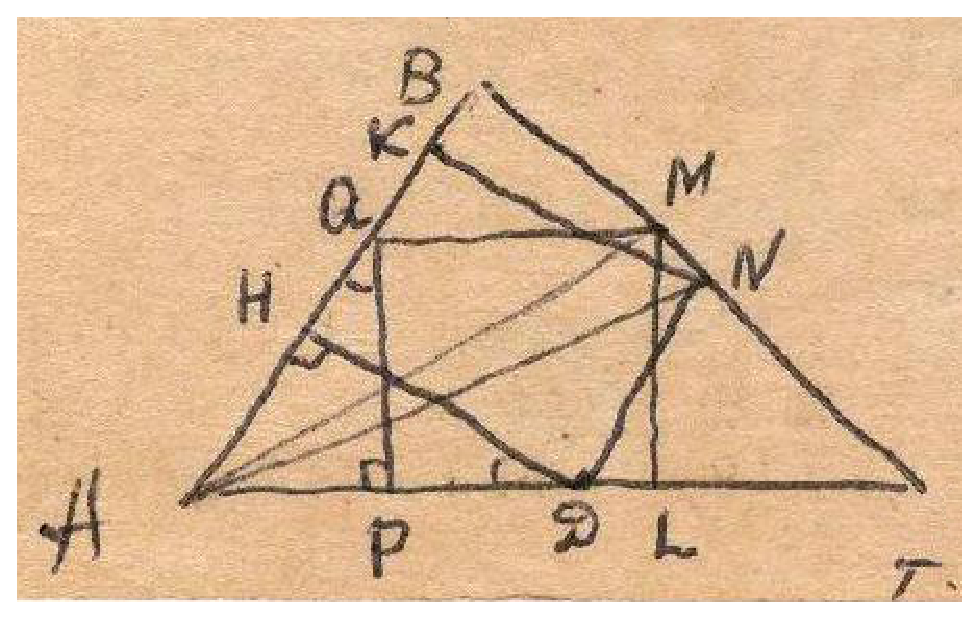
\includegraphics[width=\textwidth]{Card_T_Fig6_1.eps}
\end{minipage}\quad 	
\begin{minipage}{7cm}
	Все квадраты, вписанные в треугольник (вершины на сторонах треугольника), оказались равными. Найдите углы треугольника.
\end{minipage}

\underline{Решение:}

У каждого треугольниа $ABC$ по крайней мере два острых угла. Покажем, что если угол $A$ острый, то в условиях задачи $AB=AC$. Действительно, пусть $PQML$ и $HDNK$ -- равные квадраты. Тогда $\triangle ADH = \triangle AQP$ и следовательно $\triangle ADN = \triangle AQM$ и $\angle NDC=\angle MQB$.

С другой стороны $\angle QMC = \angle DNB$, и значит $\angle DNC = \angle QM?$. Так как и $DN=MQ$, то  $\triangle DNC = \triangle QMB$ и $AB=AC$. Если у треугольника $ABC$ еще и угол $C$ острый, то $AC=??$, т.е., треугольник равносторонний и все углы у него равны $60^{\circ}$.

\bigskip
\selectlanguage{english}
\noindent\textbf{Card T Fig 07}
\medskip
\selectlanguage{russian}

\noindent 	
\begin{minipage}{6cm}
	Можно ли на плоскости нарисовать 12 окружностей так, чтобы каждая касалась ровно 5 окружностей?
\end{minipage} \quad
\begin{minipage}{6cm}
	\underline{Подсказка: Да.}	
	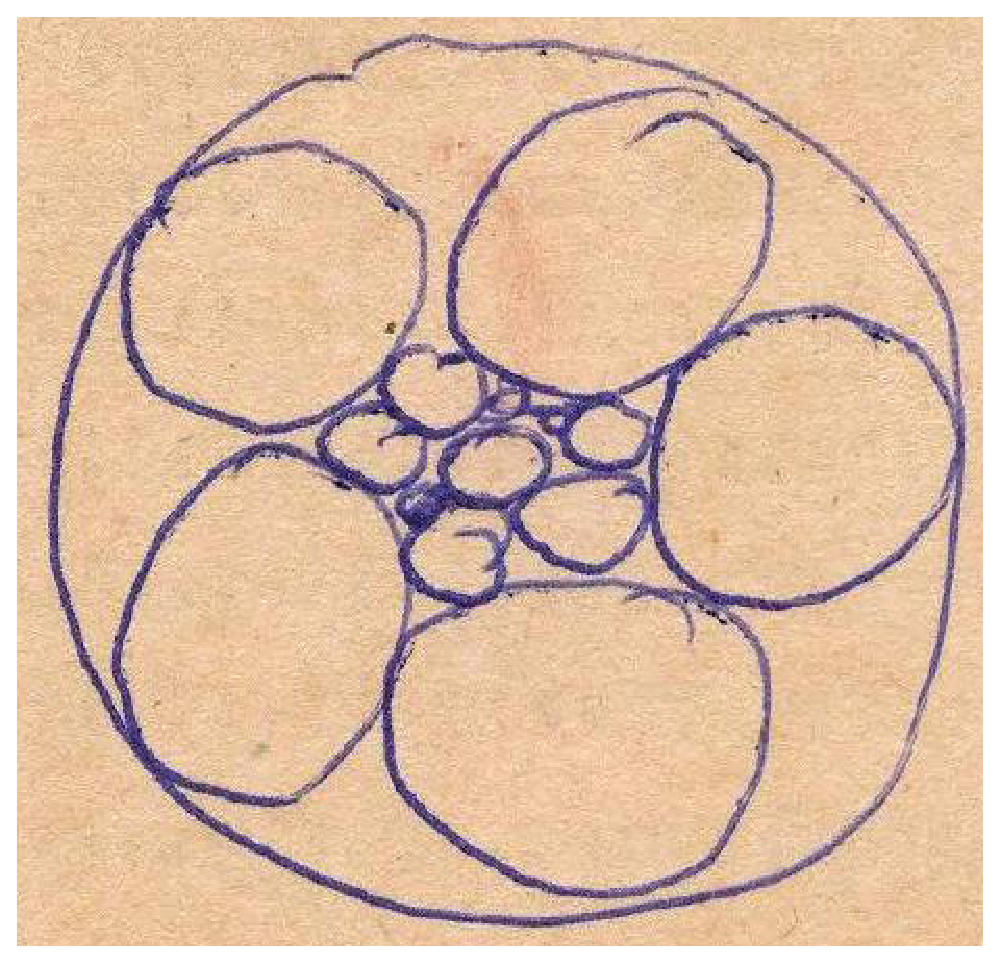
\includegraphics[width=\textwidth]{Card_T_Fig7_1.eps}
\end{minipage}


\bigskip
\selectlanguage{english}
	\noindent\textbf{Card T Fig 08}
\medskip
\selectlanguage{russian}


Через произвольную точку $P$ медианы $AD$ треугольника $\bigtriangleup ABC$ проведена прямая $B P$, пересекающая сторону $AC$ в точке $E$.

Докажите, что $AP : PD=2\cdot A E : EC$.

\underline{Подсказка:}

\noindent \begin{minipage}{6cm}
	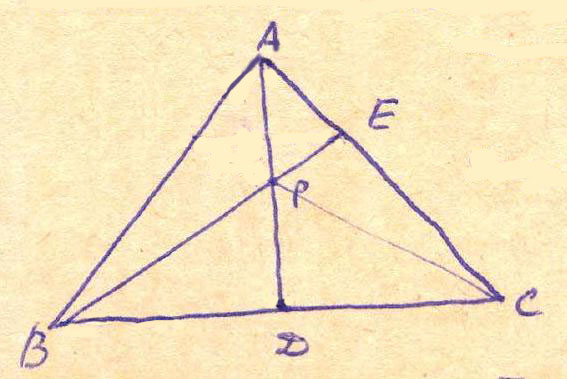
\includegraphics[width=\textwidth]{T_Fig_8.jpg}
\end{minipage}\quad 	
\begin{minipage}{7cm}
	Проведем $CP$. Тогда $S_{A B P}=S_{A C P}$ и $A E: E C=\frac{S_{A B P}}{S_{B C P}}=\frac{S_{A C P}}{S_{B C P}}= \frac{S_{A C P}}{2 S_{D P C}}=$
	$=\frac{1}{2}\cdot \frac{AP}{PD}$ 
	
	ч. и т.д.
\end{minipage}

\bigskip
\selectlanguage{english}
\noindent\textbf{Card T Fig 10}
\medskip
\selectlanguage{russian}

Через вершины треугольника проведены касательные к описанной около него окружности. Расстояния от произвольной точки окружности до прямых, содержащих стороны треугольника, обозначены через $a$, $b$, $c$, а до касательных -- $x$, $y$, $z$. Докажите, что $a^2+b^2+c^2=xy+yz+zx$.

\underline{Подсказка:}

\noindent \begin{minipage}{5cm}
	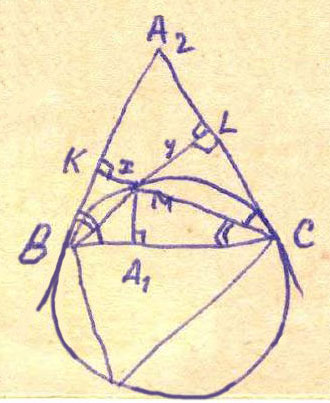
\includegraphics[width=\textwidth]{T_Fig_10.jpg}
\end{minipage}\quad 	
\begin{minipage}{8cm}
	Пусть $M$ -- точка на описанной окружности: $MK \perp BA_2$, 
	$ML \perp CA_2$, $MA_1 \perp BC$ и $MK=x$, $ML=y$, $MA_1=a$. Покажем, что $a^2=xy$. Действительно, $\bigtriangleup BMA_1\sim \bigtriangleup CML \Rightarrow	\frac{a}{y}=\frac{BM}{MC}$. Из $\bigtriangleup CMA_1\sim \bigtriangleup BMK \Rightarrow	\frac{x}{a}=\frac{BM}{MC}$. Поэтому, $\frac{a}{y}=\frac{x}{a} \Rightarrow a^2=xy$. Аналогично $b^2=yz$ и $c^2=zx$ и
	
	$a^2+b^2+c^2=xy+yz+zx$ ч. и т.д. 
	
\end{minipage}


\end{document}